\section{Methods}

\subsection{Data}

Data from this project were assembled from 22 projects on leaf spectra and related foliar traits (Table~\ref{tab:projectinfo}).
Most of these datasets are obtained directly from the ECOSIS spectral library (https://ecosis.org/).
% * <dietze@bu.edu> 2018-04-11T12:48:09.434Z:
% 
% feels like it needs a short explanation of where the rest of the spectra came from.
% 
% ^.
Collectively, these data are comprised of nearly 12,000 observations from 346 species, and span a wide geographic (Figure~\ref{fig:datamap}) and climatic range (Figure~\ref{fig:dataclimate}).

%TODO: Maybe a summary of experimental treatments?
% Milkweed stress

\begin{table}
    \caption{Project information}
    \centering
    \begin{table}[H]
\centering\begingroup\fontsize{8}{10}\selectfont

\begin{tabular}{l>{\raggedright\arraybackslash}p{25em}rrr}
\toprule
Short name & Long name & Samples & Species & Sites\\
\midrule
ACCP & Accelerated Canopy Chemistry Program (ACCP) & 850 & 46 & 5\\
ANGERS & Angers, France spectra from INRA & 274 & 37 & 1\\
Barnes 2017 & Barnes et al. 2017. Beyond greenness: Detecting temporal changes in photosynthetic capacity with hyperspectral reflectance data. PLoS ONE. & 86 & 1 & 1\\
Cali. Eco. Traits & Fresh Leaf Spectra to Estimate Leaf Traits for California Ecosystems & 261 & 16 & 34\\
Cedar Creek Biodiv. & 2014 Cedar Creek ESR Grassland Biodiversity Experiment: Leaf-level Contact Data: Trait Predictions & 780 & 18 & 1\\
\addlinespace
Corn var. & Spectral Characterization of Multiple Corn Varieties: West Madison Agricultural Station 2014 & 288 & 1 & 1\\
Di Vittorio 2009 & Di Vittorio 2009 & 504 & 2 & 3\\
Hawaii 2000 & Hawaii 2000 vegetation species spectra & 588 & 56 & 48\\
LOPEX & Leaf Optical Properties Experiment (1993) & 66 & 45 & 1\\
Milkweed stress & Common Milkweed Leaf Responses to Water Stress and Elevated Temperature & 735 & 1 & 1\\
\addlinespace
Missoula TS & Missoula Montana lodgepole pine \& big sagebrush time series & 100 & 2 & 4\\
NASA FFT & NASA Forest Functional Types (FFT) & 1369 & 66 & 130\\
NASA HyspIRI & NASA HyspIRI field campaign & 1704 & 38 & 12\\
NGEE Arctic & Next Generation Ecosystem Experiment (NGEE) - Arctic & 614 & 13 & 3\\
NGEE Tropics & Next Generation Ecosystem Experiment (NGEE) - Tropics & 706 & 28 & 1\\
\addlinespace
Pepper K/N & Fresh and Dry Pepper Leaf Spectra with Associated Potassium and Nitrogen Measurements & 119 & 1 & 1\\
PVY solanum & Varietal Discrimination and Detection of PVY in Solanum tuberosum: Hawaii 2014 & 761 & 1 & 1\\
Santa Monica Mtns. & Santa Monica Mountains vegetation species spectra & 353 & 24 & 1\\
Soybean aphid & Productivity and Characterization of Soybean Foliar Traits Under Aphid Pressure & 1131 & 1 & 1\\
Spectral variation & Spectral Variation Between Leaf-level and Canopy-level Measurements & 16 & 1 & 1\\
\addlinespace
Wu 2016 & Wu et al. 2016 New Phytologist canopy traits study & 160 & 17 & 1\\
Yang 2016 & Yang et al. 2016 Remote Sensing of Environment & 497 & 3 & 2\\
\bottomrule
\end{tabular}\endgroup{}
\end{table}
\label{tab:projectinfo}
\end{table}

\begin{figure}
    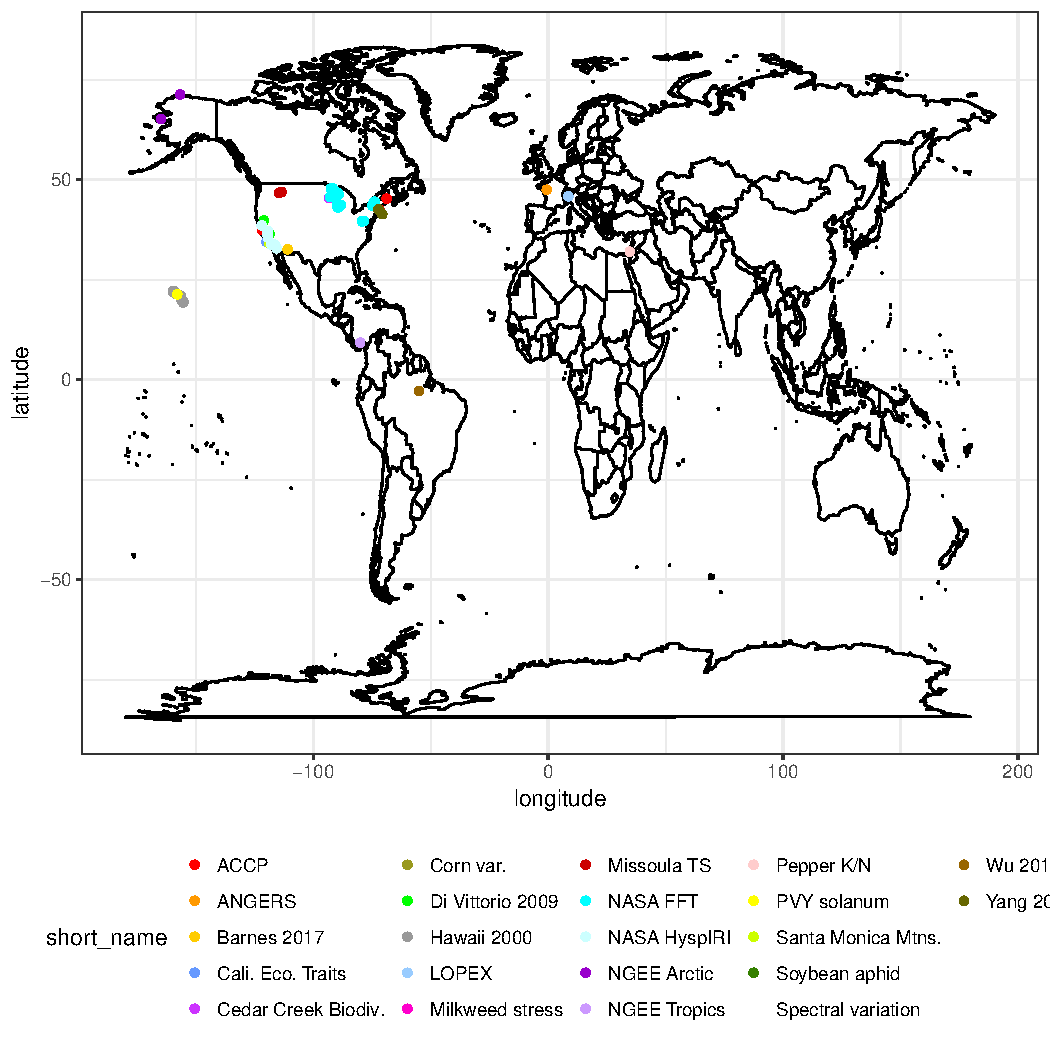
\includegraphics[width=\textwidth]{{figures/data_map}.pdf}
    \caption{Map of data locations}\label{fig:datamap}
\end{figure}
% * <dietze@bu.edu> 2018-04-11T12:49:32.972Z:
% 
% Caption is too short. Locations are getting lost among national boarders -- they need to pop out more. Legend is getting clipped and "short_name" is unnessisary
% 
% ^.

\begin{figure}
    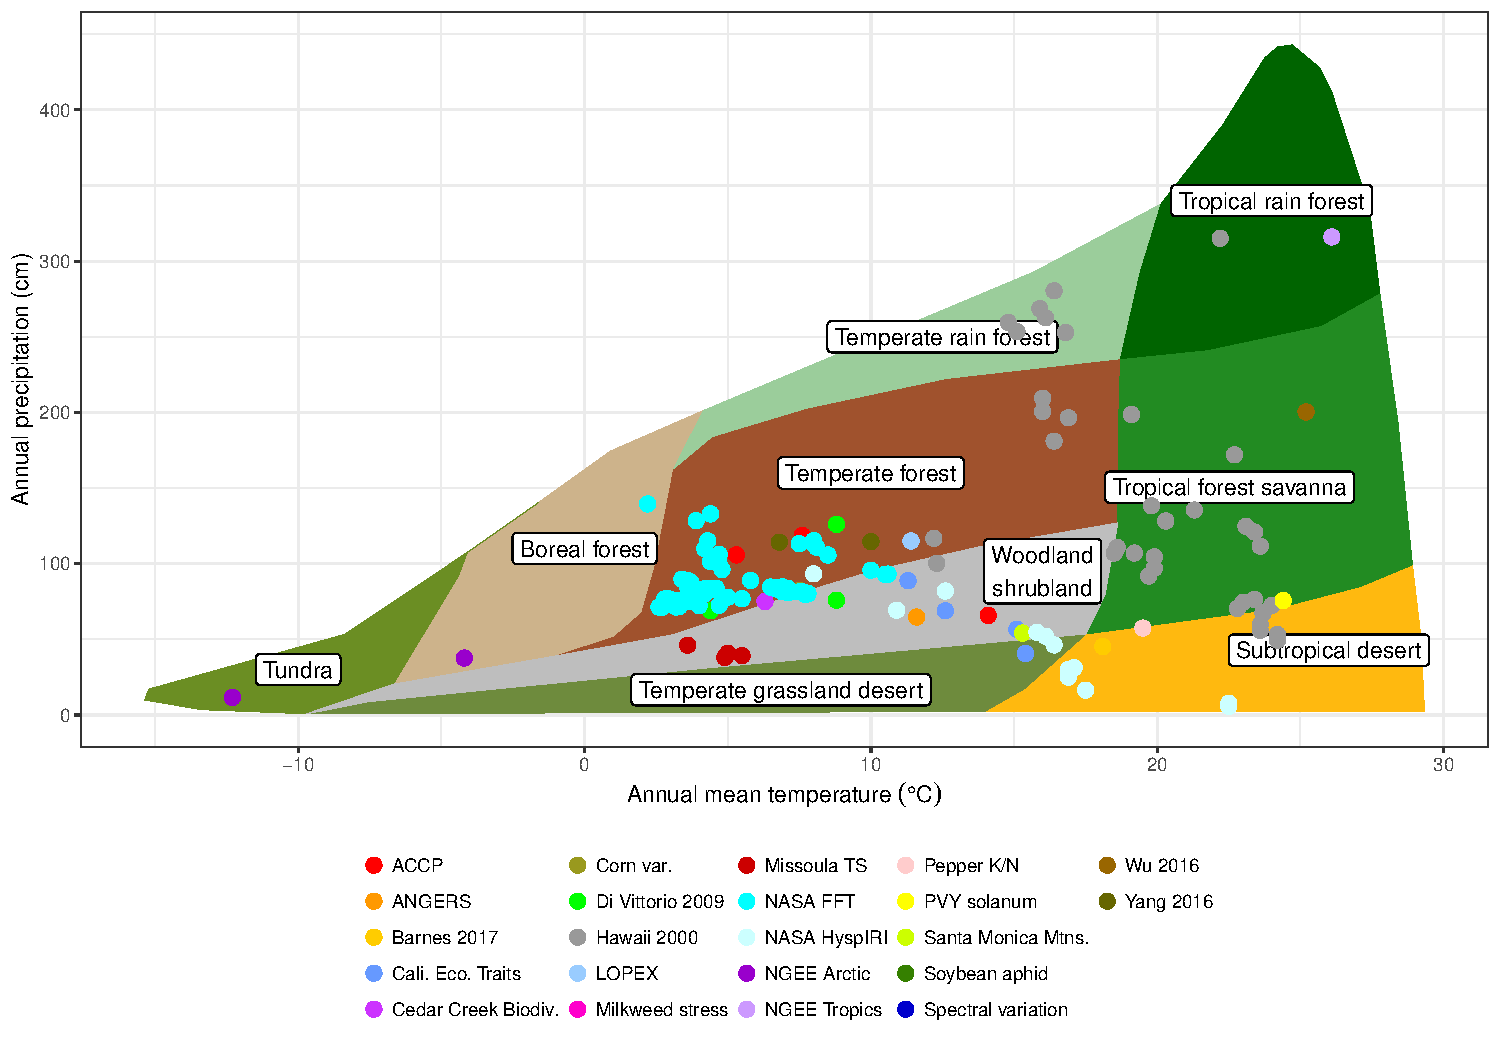
\includegraphics[width=\textwidth]{{figures/data_climate}.pdf}
    \caption{Data locations in climate space}\label{fig:dataclimate}
\end{figure}
% * <dietze@bu.edu> 2018-04-11T12:54:27.768Z:
% 
% Points too small. Precip units are wrong (y-axis is in cm)
% 
% ^.

\subsection{Trait estimation via PROSPECT inversion}

\begin{figure}
  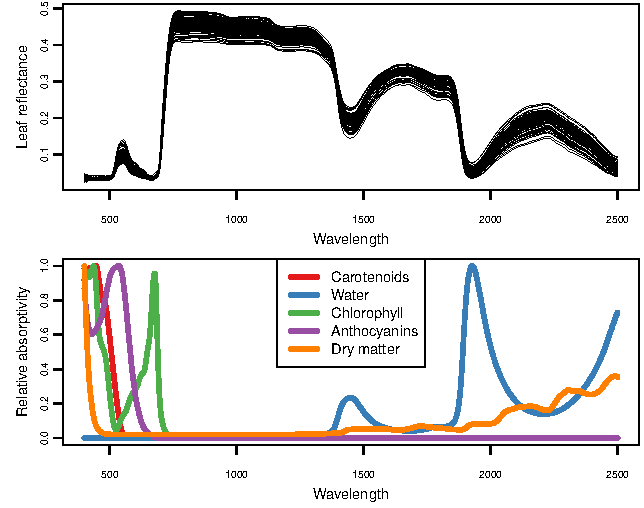
\includegraphics[width=\textwidth]{{figures/sigspec2-1}.pdf}
  \caption{\
    (Top) Example reflectance spectra of \textit{Acer rubrum} leaves.
    (Bottom) Normalized absorption coefficients for traits estimated by PROSPECT.
  }\label{fig:prospect_coefficients}
\end{figure}
% * <dietze@bu.edu> 2018-04-11T12:58:55.715Z:
% 
% Minor point, but would it be easier to visually see the relationship between the overall specta and the traits if the prospect coefficients were graphed in terms of reflectance instead of absorption?
% 
% ^.

The PROSPECT leaf radiative transfer model~\cite{jacquemoud1990_prospect,jacquemoud_2009_prosail,feret2008_prospect,feret2017_prospectd} simulates leaf reflectance and transmittance for 400 to 2500 nm wavelengths at 1 nm increments as a function of leaf morphological and biochemical characteristics.
In this chapter, I compared the performance of four different versions of PROSPECT, each of which uses a different combination of leaf traits:
PROSPECT 4 uses
total chlorophyll content per area ($\mu g~cm^{-2}$),
leaf water content per area ($g~m^{-2}$),
and leaf dry matter content per area ($g~m^{-2}$)~\cite{feret2008_prospect}.
PROSPECT 5 extends PROSPECT 4 with a parameter for
total carotenoid content per area ($\mu g~cm^{-2}$)~\cite{feret2008_prospect}.
PROSPECT 5B adds an additional parameter for
total ``senescent brown pigment'' content (arbitrary units)~\cite{jacquemoud_2009_prosail}.
Finally, PROSPECT D adds an additional parameter for
total anthocynanin content per area ($\mu g~cm^{-2}$)~\cite{feret2017_prospectd}.
The absorption coefficients for PROSPECT-D aligned with example leaf reflectance spectra are shown in Figure~\ref{fig:prospect_coefficients}.

To estimate traits from leaf spectra, I generally followed the Bayesian RTM inversion approach of~\cite{shiklomanov2016_rse}, except that I replaced the Metropolis-Hastings algorithm with a more efficient Differential Evolution algorithm with ``snooker'' update as implemented in the \texttt{BayesianTools} R package~\cite{bayesiantools}.
Forward simulations and Bayesian inversion of PROSPECT are implemented in the R package \texttt{PEcAnRTM}~\cite{shiklomanov2016_rse}, which is open source and freely available at https://github.com/pecanproject/pecan/modules/rtm.
Where leaf spectra extended beyond the 400 to 2500 nm wavelength range of the PROSPECT model, I used only the observations from 400 to 2500 nm.
Where leaf spectra were sampled at a spectral resolution coarser than 1 nm or did not include all wavelengths simulated by PROSPECT, I subset the PROSPECT output in the likelihood function to match the observations.
Where leaf spectra were sampled at a finer spectral resolution than 1 nm, or where wavelengths did not align at 1 nm intervals, I used cubic spline interpolation (default method in the base R function \texttt{spline}) to align the spectra with PROSPECT output.
Where leaf spectra were provided as ``pseudo-absorbance'' ($1 - \log_{10}(R)$), I added the corresponding transformation to the PROSPECT output in the likelihood calculation. 

\subsection{Analysis}

To compare PROSPECT versions, I plotted traits estimated by more than one version of PROSPECT as pairwise scatter plots, fit a least-squares linear regression to each and compared the result to a 1-to-1 line, and calculated the pairwise correlation coefficient (Figures~\ref{fig:prospect_pairs_N}-\ref{fig:prospect_pairs_Cm}).
% * <dietze@bu.edu> 2018-04-11T13:01:34.687Z:
% 
% > more than one version of PROSPECT as pairwise scatter plots
% This specific bit is confusing, and the overall sentence is a run-on.
% 
% ^.
To validate PROSPECT inversions, I compared trait estimates from PROSPECT inversion with direct measurements of the corresponding traits, where these traits were available.
To explore project-specific biases in the inversion, I fit least-squares linear regressions to investigate the ability of trait estimates from spectra to predict the measured traits, and I report the slopes, intercepts, and $R^2$ values of those regressions (Figure~\ref{fig:project_validation_summary}, Supplementary Tables~\ref{tab:r2_byproject_Cab}-\ref{tab:r2_byproject_Cm}).
To identify species-specific errors, I also performed this analysis for each project-species combination with at least 5 observations (Figures~\ref{fig:error_speciesbyproj_Cab}-\ref{fig:error_speciesbyproj_Cm}).

To investigate the effects of experimental treatments and environmental conditions, I fit a linear fixed effects model for each optical trait and each treatment, with an additional fixed effect for species if multiple species were present in that treatment.
To investigate the role of intraspecific variability in climate, I subset the data to species that were present at at least 10 different sites and fit a fixed-effects model to each optical trait as a function of species, annual mean temperature, and annual precipitation.
I then present the direction of each GLM coefficient and whether the coefficient was significant (Figure~\ref{fig:treatment_summary}).

One study in this dataset---Yang et al.~(2016) \nocite{yang_2016_seasonal}---explicitly looked at the seasonal trajectories of leaf reflectance, allowing me the chance to look at the phenology of leaf optical traits (Figure~\ref{fig:trait_phenology}).

To investigate the correlations between optical traits and other traits measured directly, I calculated the pairwise non-missing correlations (R function \texttt{cor} with option \texttt{use = pairwise.complete.obs}) and plotted the resulting correlation coefficients using the \texttt{corrplot} package.
I performed this analysis for both individual observations and species means, where a trait was observed for at least 3 species.

I performed all analyses using R version 3.4.4~\cite{rstats}.
The data and code for performing these analyses are open source and freely available at https://github.com/ashiklom/rspecan.
